% Options for packages loaded elsewhere
\PassOptionsToPackage{unicode}{hyperref}
\PassOptionsToPackage{hyphens}{url}
%
\documentclass[
]{article}
\usepackage{amsmath,amssymb}
\usepackage{lmodern}
\usepackage{iftex}
\ifPDFTeX
  \usepackage[T1]{fontenc}
  \usepackage[utf8]{inputenc}
  \usepackage{textcomp} % provide euro and other symbols
\else % if luatex or xetex
  \usepackage{unicode-math}
  \defaultfontfeatures{Scale=MatchLowercase}
  \defaultfontfeatures[\rmfamily]{Ligatures=TeX,Scale=1}
\fi
% Use upquote if available, for straight quotes in verbatim environments
\IfFileExists{upquote.sty}{\usepackage{upquote}}{}
\IfFileExists{microtype.sty}{% use microtype if available
  \usepackage[]{microtype}
  \UseMicrotypeSet[protrusion]{basicmath} % disable protrusion for tt fonts
}{}
\makeatletter
\@ifundefined{KOMAClassName}{% if non-KOMA class
  \IfFileExists{parskip.sty}{%
    \usepackage{parskip}
  }{% else
    \setlength{\parindent}{0pt}
    \setlength{\parskip}{6pt plus 2pt minus 1pt}}
}{% if KOMA class
  \KOMAoptions{parskip=half}}
\makeatother
\usepackage{xcolor}
\usepackage[margin=1in]{geometry}
\usepackage{graphicx}
\makeatletter
\def\maxwidth{\ifdim\Gin@nat@width>\linewidth\linewidth\else\Gin@nat@width\fi}
\def\maxheight{\ifdim\Gin@nat@height>\textheight\textheight\else\Gin@nat@height\fi}
\makeatother
% Scale images if necessary, so that they will not overflow the page
% margins by default, and it is still possible to overwrite the defaults
% using explicit options in \includegraphics[width, height, ...]{}
\setkeys{Gin}{width=\maxwidth,height=\maxheight,keepaspectratio}
% Set default figure placement to htbp
\makeatletter
\def\fps@figure{htbp}
\makeatother
\setlength{\emergencystretch}{3em} % prevent overfull lines
\providecommand{\tightlist}{%
  \setlength{\itemsep}{0pt}\setlength{\parskip}{0pt}}
\setcounter{secnumdepth}{-\maxdimen} % remove section numbering
\usepackage{multirow}
\usepackage{multicol}
\usepackage{colortbl}
\usepackage{hhline}
\newlength\Oldarrayrulewidth
\newlength\Oldtabcolsep
\usepackage{longtable}
\usepackage{array}
\usepackage{hyperref}
\usepackage{float}
\usepackage{wrapfig}
\ifLuaTeX
  \usepackage{selnolig}  % disable illegal ligatures
\fi
\IfFileExists{bookmark.sty}{\usepackage{bookmark}}{\usepackage{hyperref}}
\IfFileExists{xurl.sty}{\usepackage{xurl}}{} % add URL line breaks if available
\urlstyle{same} % disable monospaced font for URLs
\hypersetup{
  pdftitle={Black Sea Bass () Ecosystem \& Socioeconomic Profile Report Card},
  hidelinks,
  pdfcreator={LaTeX via pandoc}}

\title{Black Sea Bass (\protect\textit{Centropristis striata})
\protect\newline Ecosystem \& Socioeconomic Profile Report Card}
\author{}
\date{\vspace{-2.5em}}

\begin{document}
\maketitle

\vspace{-2.5cm}
\section{Spring 2025}

Black sea bass is an important Mid-Atlantic stock with high commercial
value and recreational engagement. There are two stock subunits, divided
at the Hudson Canyon. Overfishing is not occurring and the stock is not
overfished. The stock assessment model uses winter bottom temperature as
a recruitment covariate to incorporate the observed link between cold
temperature and smaller year classes.

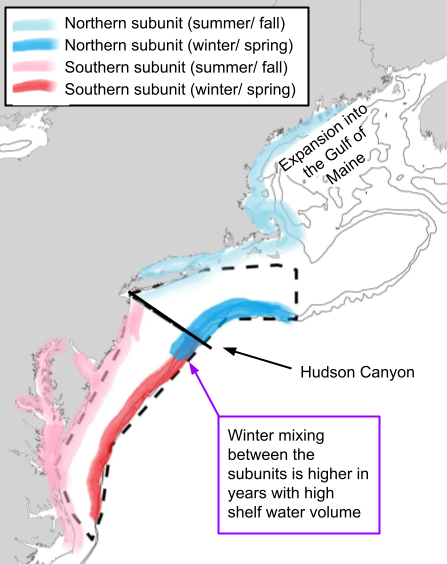
\includegraphics{/home/atyrell/SOE_ESP_Data/bsb/images/bsb_map.png}

\hfill

\section{2024 in Review}

\subsection{Fishing Community Observations}

\begin{itemize}
\tightlist
\item
  Steady or increasing availability
\item
  Expanding distributions and changes in migration timing
\item
  Local regulatory complexity affects fishing opportunities
\end{itemize}

\subsection{Commercial Fishery}

\begin{itemize}
\tightlist
\item
  Number of active vessels declined in 2024, but total landed pounds
  increased from 2023 and have been following an overall increasing
  trend over the last decade
\item
  Total revenue decreased slightly along with average prices (\$/lb)
\item
  Average revenue per vessel increased, following an upward trend over
  the past three years for vessels that remain in the fishery as the
  number of active vessels continues to decline
\end{itemize}

\subsection{Recreational Fishery}

\begin{itemize}
\tightlist
\item
  Number of targeted trips, catch, and landings all down from 2023
\item
  But number of trips still above the historic average
\item
  Not clear if catch per angler has continued to increase in 2024
\end{itemize}

\subsection{Ecosystem}

\begin{itemize}
\tightlist
\item
  Cold winter in the north but near average in the south
\item
  Poor or below average fish condition in recent years
\end{itemize}

\vspace{0.5cm}
\section{Key Points from the Mid-Atlantic Risk Assessment}

\vspace{-3cm}

\raggedright

According to the
\href{https://static1.squarespace.com/static/511cdc7fe4b00307a2628ac6/t/6747560a3cf66936045e5547/1732728332670/05_EAFM+Risk+Assessment.pdf}{Mid-Atlantic
2024 EAFM risk assessment update}, Black Sea Bass scored high and/or
moderately high risk in the following elements:

\begin{itemize}
\tightlist
\item
  Moderate-high to high risk to the stock due to:

  \begin{itemize}
  \tightlist
  \item
    Very high exposure to changes in climate
  \item
    Observed and potential changes in distribution; northward shift into
    the Gulf of Maine
  \item
    Dependence on threatened estuarine habitat
  \item
    Decline in the biomass of benthic invertebrate prey
  \item
    Decline in black sea bass body condition in the Mid Atlantic Bight
  \end{itemize}
\item
  High risk to the recreational fishery due to:

  \begin{itemize}
  \tightlist
  \item
    Catch exceeding harvest limits in several years
  \item
    High regulatory complexity; frequent changes and varying interstate
    regulations; regulatory changes in allocations
  \end{itemize}
\item
  Moderate-high risk to the commercial fishery due to:

  \begin{itemize}
  \tightlist
  \item
    Commercial revenue in wind development areas
  \item
    High discards \& discard mortality
  \end{itemize}
\end{itemize}

\hfill

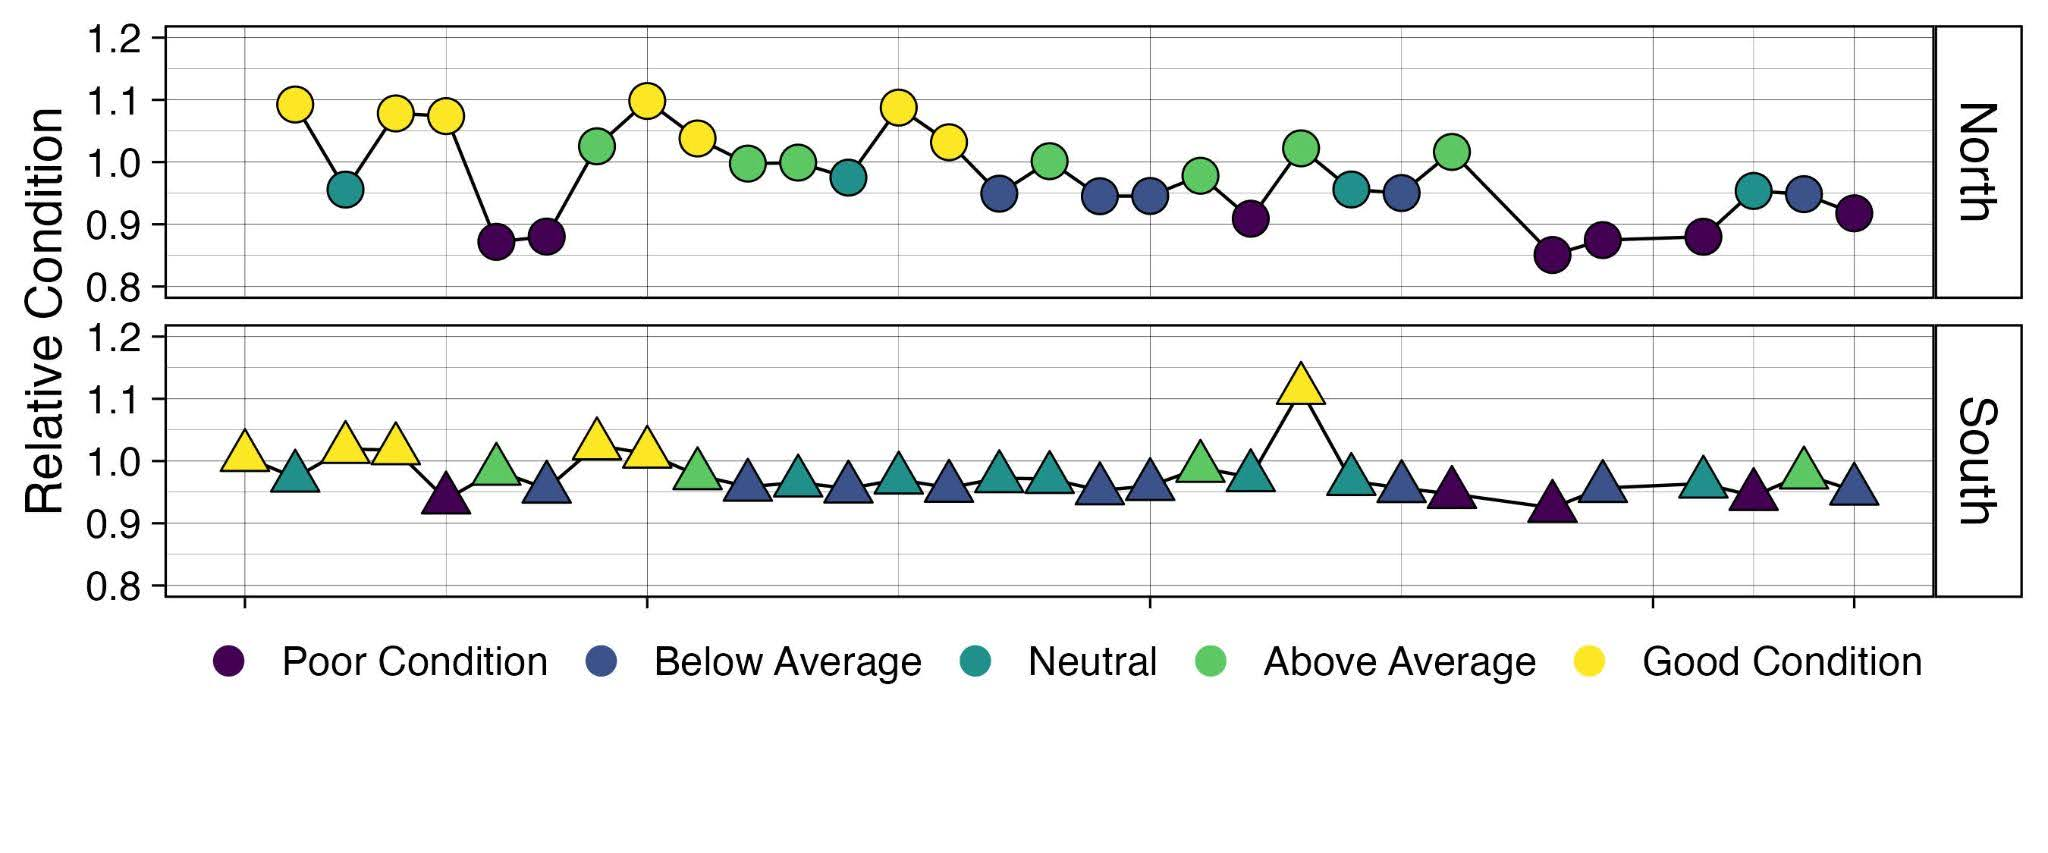
\includegraphics{/home/atyrell/SOE_ESP_Data/bsb/images/condition.jpg}
\includegraphics{list(level = c(4, 4, 4, 3, 3, 3, 2, 2, 2, 1, 1, 1), name = c("stock", "commercial", "recreational", "stock", "commercial", "recreational", "stock", "commercial", "recreational", "stock", "commercial", "recreational"), value = c(2, 0, 3, 2, 2, 1, 0, 4, 1, 4, 1, 1), percent = c(0.25, 0, 0.5, 0.25, 0.285714285714286, 0.166666666666667, 0, 0.571428571428571, 0.166666666666667, 0.5, 0.142857142857143, 0.166666666666667), lab = c("2 Low", NA, "3 Low", "2 Lowmod", "2 Lowmod", "1 Lowmod", NA, "4 Modhigh", "1 Modhigh", "4 High", "1 High", "1 High"), pos = c(0.25, 0, 0.5, 0.5, 0.285714285714286, 0.666666666666667, 0.5, 0.857142857142857, 0.833333333333333, 1, 1, 1), xlab = c("Stock/n(8 Risk Elements)", "Commercial/n(7 Risk Elements)", "Recreational/n(6 Risk Elements)", "Stock/n(8 Risk Elements)", "Commercial/n(7 Risk Elements)", "Recreational/n(6 Risk Elements)", "Stock/n(8 Risk Elements)", "Commercial/n(7 Risk Elements)", "Recreational/n(6 Risk Elements)", "Stock/n(8 Risk Elements)", "Commercial/n(7 Risk Elements)", "Recreational/n(6 Risk Elements)"), .group = c(3, 1, 2, 3, 1, 2, 3, 1, 2, 3, 1, 2)), list(\textless{}environment\textgreater{}, \textless{}environment\textgreater{}, \textless{}environment\textgreater{}), \textless{}environment\textgreater{}, \textless{}environment\textgreater{}, list(x = ~xlab, y = ~percent, fill = ~level), list(line = list(colour = "black", linewidth = 0.5, linetype = 1, lineend = "butt", arrow = FALSE, inherit.blank = TRUE), rect = list(fill = "white", colour = "black", linewidth = 0.5, linetype = 1, inherit.blank = TRUE), text = list(family = "", face = "plain", colour = "black", size = 11, hjust = 0.5, vjust = 0.5, angle = 0, lineheight = 0.9, margin = c(0, 0, 0, 0), debug = FALSE, inherit.blank = TRUE), title = NULL, aspect.ratio = NULL, axis.title = NULL, axis.title.x = list(), axis.title.x.top = list( family = NULL, face = NULL, colour = NULL, size = NULL, hjust = NULL, vjust = 0, angle = NULL, lineheight = NULL, margin = c(0, 0, 2.75, 0), debug = NULL, inherit.blank = TRUE), axis.title.x.bottom = NULL, axis.title.y = list(family = NULL, face = NULL, colour = NULL, size = NULL, hjust = NULL, vjust = 1, angle = 90, lineheight = NULL, margin = c(0, 2.75, 0, 0), debug = NULL, inherit.blank = TRUE), axis.title.y.left = NULL, axis.title.y.right = list(family = NULL, face = NULL, colour = NULL, size = NULL, hjust = NULL, vjust = 1, angle = -90, lineheight = NULL, margin = c(0, 0, 0, 2.75), debug = NULL, inherit.blank = TRUE), axis.text = list(family = NULL, face = NULL, colour = "grey30", size = 0.8, hjust = NULL, vjust = NULL, angle = NULL, lineheight = NULL, margin = NULL, debug = NULL, inherit.blank = TRUE), axis.text.x = list(), axis.text.x.top = list(family = NULL, face = NULL, colour = NULL, size = NULL, hjust = NULL, vjust = 0, angle = NULL, lineheight = NULL, margin = c(0, 0, 2.2, 0), debug = NULL, inherit.blank = TRUE), axis.text.x.bottom = NULL, axis.text.y = list(family = NULL, face = NULL, colour = "black", size = NULL, hjust = 1, vjust = NULL, angle = NULL, lineheight = NULL, margin = c(0, 2.2, 0, 0), debug = NULL, inherit.blank = FALSE), axis.text.y.left = NULL, axis.text.y.right = list(family = NULL, face = NULL, colour = NULL, size = NULL, hjust = 0, vjust = NULL, angle = NULL, lineheight = NULL, margin = c(0, 0, 0, 2.2), debug = NULL, inherit.blank = TRUE), axis.text.theta = NULL, axis.text.r = list(family = NULL, face = NULL, colour = NULL, size = NULL, hjust = 0.5, vjust = NULL, angle = NULL, lineheight = NULL, margin = c(0, 2.2, 0, 2.2), debug = NULL, inherit.blank = TRUE), axis.ticks = list(), axis.ticks.x = NULL, axis.ticks.x.top = NULL, axis.ticks.x.bottom = NULL, axis.ticks.y = NULL, axis.ticks.y.left = NULL, axis.ticks.y.right = NULL, axis.ticks.theta = NULL, axis.ticks.r = NULL, axis.minor.ticks.x.top = NULL, axis.minor.ticks.x.bottom = NULL, axis.minor.ticks.y.left = NULL, axis.minor.ticks.y.right = NULL, axis.minor.ticks.theta = NULL, axis.minor.ticks.r = NULL, axis.ticks.length = 2.75, axis.ticks.length.x = NULL, axis.ticks.length.x.top = NULL, axis.ticks.length.x.bottom = NULL, axis.ticks.length.y = NULL, axis.ticks.length.y.left = NULL, axis.ticks.length.y.right = NULL, axis.ticks.length.theta = NULL, axis.ticks.length.r = NULL, axis.minor.ticks.length = 0.75, axis.minor.ticks.length.x = NULL, axis.minor.ticks.length.x.top = NULL, axis.minor.ticks.length.x.bottom = NULL, axis.minor.ticks.length.y = NULL, axis.minor.ticks.length.y.left = NULL, axis.minor.ticks.length.y.right = NULL, axis.minor.ticks.length.theta = NULL, axis.minor.ticks.length.r = NULL, axis.line = list(), axis.line.x = NULL, axis.line.x.top = NULL, axis.line.x.bottom = NULL, axis.line.y = NULL, axis.line.y.left = NULL, axis.line.y.right = NULL, axis.line.theta = NULL, axis.line.r = NULL, legend.background = list(fill = NULL, colour = NA, linewidth = NULL, linetype = NULL, inherit.blank = TRUE), legend.margin = c(5.5, 5.5, 5.5, 5.5), legend.spacing = 11, legend.spacing.x = NULL, legend.spacing.y = NULL, legend.key = NULL, legend.key.size = 1.2, legend.key.height = NULL, legend.key.width = NULL, legend.key.spacing = 5.5, legend.key.spacing.x = NULL, legend.key.spacing.y = NULL, legend.frame = NULL, legend.ticks = NULL, legend.ticks.length = 0.2, legend.axis.line = NULL, legend.text = list(family = NULL, face = NULL, colour = NULL, size = 0.8, hjust = NULL, vjust = NULL, angle = NULL, lineheight = NULL, margin = NULL, debug = NULL, inherit.blank = TRUE), legend.text.position = NULL, legend.title = list(family = NULL, face = NULL, colour = NULL, size = NULL, hjust = 0, vjust = NULL, angle = NULL, lineheight = NULL, margin = NULL, debug = NULL, inherit.blank = TRUE), legend.title.position = NULL, legend.position = "none", legend.position.inside = NULL, legend.direction = NULL, legend.byrow = NULL, legend.justification = "center", legend.justification.top = NULL, legend.justification.bottom = NULL, legend.justification.left = NULL, legend.justification.right = NULL, legend.justification.inside = NULL, legend.location = NULL, legend.box = NULL, legend.box.just = NULL, legend.box.margin = c(0, 0, 0, 0), legend.box.background = list(), legend.box.spacing = 11, panel.background = list(fill = "white", colour = NA, linewidth = NULL, linetype = NULL, inherit.blank = TRUE), panel.border = list(), panel.spacing = 5.5, panel.spacing.x = NULL, panel.spacing.y = NULL, panel.grid = list(colour = "grey92", linewidth = NULL, linetype = NULL, lineend = NULL, arrow = FALSE, inherit.blank = TRUE), panel.grid.major = list(), panel.grid.minor = list(), panel.grid.major.x = NULL, panel.grid.major.y = list(colour = "gray", linewidth = NULL, linetype = NULL, lineend = NULL, arrow = FALSE, inherit.blank = FALSE), panel.grid.minor.x = NULL, panel.grid.minor.y = NULL, panel.ontop = FALSE, plot.background = list(fill = NULL, colour = "white", linewidth = NULL, linetype = NULL, inherit.blank = TRUE), plot.title = list( family = NULL, face = NULL, colour = NULL, size = 1.2, hjust = 0, vjust = 1, angle = NULL, lineheight = NULL, margin = c(0, 0, 5.5, 0), debug = NULL, inherit.blank = TRUE), plot.title.position = "panel", plot.subtitle = list(family = NULL, face = NULL, colour = NULL, size = NULL, hjust = 0, vjust = 1, angle = NULL, lineheight = NULL, margin = c(0, 0, 5.5, 0), debug = NULL, inherit.blank = TRUE), plot.caption = list(family = NULL, face = NULL, colour = NULL, size = 0.8, hjust = 1, vjust = 1, angle = NULL, lineheight = NULL, margin = c(5.5, 0, 0, 0), debug = NULL, inherit.blank = TRUE), plot.caption.position = "panel", plot.tag = list(family = NULL, face = NULL, colour = NULL, size = 1.2, hjust = 0.5, vjust = 0.5, angle = NULL, lineheight = NULL, margin = NULL, debug = NULL, inherit.blank = TRUE), plot.tag.position = "topleft", plot.tag.location = NULL, plot.margin = c(5.5, 5.5, 5.5, 5.5), strip.background = list(fill = "white", colour = "black", linewidth = 2, linetype = NULL, inherit.blank = TRUE), strip.background.x = NULL, strip.background.y = NULL, strip.clip = "inherit", strip.placement = "inside", strip.text = list(family = NULL, face = NULL, colour = "grey10", size = 0.8, hjust = NULL, vjust = NULL, angle = NULL, lineheight = NULL, margin = c(4.4, 4.4, 4.4, 4.4), debug = NULL, inherit.blank = TRUE), strip.text.x = NULL, strip.text.x.bottom = NULL, strip.text.x.top = NULL, strip.text.y = list(family = NULL, face = NULL, colour = NULL, size = NULL, hjust = NULL, vjust = NULL, angle = -90, lineheight = NULL, margin = NULL, debug = NULL, inherit.blank = TRUE), strip.text.y.left = list(family = NULL, face = NULL, colour = NULL, size = NULL, hjust = NULL, vjust = NULL, angle = 90, lineheight = NULL, margin = NULL, debug = NULL, inherit.blank = TRUE), strip.text.y.right = NULL, strip.switch.pad.grid = 2.75, strip.switch.pad.wrap = 2.75), \textless{}environment\textgreater{}, \textless{}environment\textgreater{}, \textless{}environment\textgreater{}, \textless{}environment\textgreater{}, list(y = "Percent of Risk Elements", x = "xlab", fill = "level", label = "lab")}

\newpage

\newgeometry{top=0.25in, left=0.25in, right=0.25in, bottom=0.25in}

\begin{verbatim}
## Warning: fonts used in `flextable` are ignored because the `pdflatex` engine is
## used and not `xelatex` or `lualatex`. You can avoid this warning by using the
## `set_flextable_defaults(fonts_ignore=TRUE)` command or use a compatible engine
## by defining `latex_engine: xelatex` in the YAML header of the R Markdown
## document.
\end{verbatim}

\global\setlength{\Oldarrayrulewidth}{\arrayrulewidth}

\global\setlength{\Oldtabcolsep}{\tabcolsep}

\setlength{\tabcolsep}{2pt}

\renewcommand*{\arraystretch}{1.5}



\providecommand{\ascline}[3]{\noalign{\global\arrayrulewidth #1}\arrayrulecolor[HTML]{#2}\cline{#3}}

\begin{longtable}[c]{|p{0.90in}|p{0.75in}|p{3.00in}|p{3.00in}|p{0.75in}}



\hhline{>{\arrayrulecolor[HTML]{666666}\global\arrayrulewidth=0.75pt}->{\arrayrulecolor[HTML]{666666}\global\arrayrulewidth=0.75pt}->{\arrayrulecolor[HTML]{666666}\global\arrayrulewidth=0.75pt}->{\arrayrulecolor[HTML]{666666}\global\arrayrulewidth=0.75pt}->{\arrayrulecolor[HTML]{666666}\global\arrayrulewidth=0.75pt}-}

\multicolumn{1}{!{\color[HTML]{666666}\vrule width 0.75pt}>{\centering}m{\dimexpr 0.9in+0\tabcolsep}}{\textcolor[HTML]{000000}{\fontsize{10}{10}\selectfont{\textbf{Indicator\ Units}}}} & \multicolumn{1}{!{\color[HTML]{666666}\vrule width 0.75pt}>{\centering}m{\dimexpr 0.75in+0\tabcolsep}}{\textcolor[HTML]{000000}{\fontsize{10}{10}\selectfont{\textbf{Status\ In\ 2024}}}} & \multicolumn{1}{!{\color[HTML]{666666}\vrule width 0.75pt}>{\centering}m{\dimexpr 3in+0\tabcolsep}}{\textcolor[HTML]{000000}{\fontsize{10}{10}\selectfont{\textbf{Implications}}}} & \multicolumn{1}{!{\color[HTML]{666666}\vrule width 0.75pt}>{\centering}m{\dimexpr 3in+0\tabcolsep}}{\textcolor[HTML]{000000}{\fontsize{10}{10}\selectfont{\textbf{Time\ Series\ 2}}}} & \multicolumn{1}{!{\color[HTML]{666666}\vrule width 0.75pt}>{\raggedleft}m{\dimexpr 0.75in+0\tabcolsep}!{\color[HTML]{666666}\vrule width 0.75pt}}{\textcolor[HTML]{000000}{\fontsize{10}{10}\selectfont{\textbf{Time\ Series}}}} \\

\noalign{\global\arrayrulewidth 0.75pt}\arrayrulecolor[HTML]{666666}

\hhline{|>{\arrayrulecolor[HTML]{666666}\global\arrayrulewidth=0.75pt}-|>{\arrayrulecolor[HTML]{666666}\global\arrayrulewidth=0.75pt}-|>{\arrayrulecolor[HTML]{666666}\global\arrayrulewidth=0.75pt}-|>{\arrayrulecolor[HTML]{666666}\global\arrayrulewidth=0.75pt}-|>{\arrayrulecolor[HTML]{666666}\global\arrayrulewidth=0.75pt}-}\endfirsthead 

\hhline{>{\arrayrulecolor[HTML]{666666}\global\arrayrulewidth=0.75pt}->{\arrayrulecolor[HTML]{666666}\global\arrayrulewidth=0.75pt}->{\arrayrulecolor[HTML]{666666}\global\arrayrulewidth=0.75pt}->{\arrayrulecolor[HTML]{666666}\global\arrayrulewidth=0.75pt}->{\arrayrulecolor[HTML]{666666}\global\arrayrulewidth=0.75pt}-}

\multicolumn{1}{!{\color[HTML]{666666}\vrule width 0.75pt}>{\centering}m{\dimexpr 0.9in+0\tabcolsep}}{\textcolor[HTML]{000000}{\fontsize{10}{10}\selectfont{\textbf{Indicator\ Units}}}} & \multicolumn{1}{!{\color[HTML]{666666}\vrule width 0.75pt}>{\centering}m{\dimexpr 0.75in+0\tabcolsep}}{\textcolor[HTML]{000000}{\fontsize{10}{10}\selectfont{\textbf{Status\ In\ 2024}}}} & \multicolumn{1}{!{\color[HTML]{666666}\vrule width 0.75pt}>{\centering}m{\dimexpr 3in+0\tabcolsep}}{\textcolor[HTML]{000000}{\fontsize{10}{10}\selectfont{\textbf{Implications}}}} & \multicolumn{1}{!{\color[HTML]{666666}\vrule width 0.75pt}>{\centering}m{\dimexpr 3in+0\tabcolsep}}{\textcolor[HTML]{000000}{\fontsize{10}{10}\selectfont{\textbf{Time\ Series\ 2}}}} & \multicolumn{1}{!{\color[HTML]{666666}\vrule width 0.75pt}>{\raggedleft}m{\dimexpr 0.75in+0\tabcolsep}!{\color[HTML]{666666}\vrule width 0.75pt}}{\textcolor[HTML]{000000}{\fontsize{10}{10}\selectfont{\textbf{Time\ Series}}}} \\

\noalign{\global\arrayrulewidth 0.75pt}\arrayrulecolor[HTML]{666666}

\hhline{|>{\arrayrulecolor[HTML]{666666}\global\arrayrulewidth=0.75pt}-|>{\arrayrulecolor[HTML]{666666}\global\arrayrulewidth=0.75pt}-|>{\arrayrulecolor[HTML]{666666}\global\arrayrulewidth=0.75pt}-|>{\arrayrulecolor[HTML]{666666}\global\arrayrulewidth=0.75pt}-|>{\arrayrulecolor[HTML]{666666}\global\arrayrulewidth=0.75pt}-}\endhead



\multicolumn{1}{!{\color[HTML]{666666}\vrule width 0.75pt}>{\cellcolor[HTML]{FFFFFF}\raggedright}m{\dimexpr 0.9in+0\tabcolsep}}{\textcolor[HTML]{000000}{\fontsize{10}{10}\selectfont{Mean\ winter\ (Feb-Mar)\ bottom\ temperature\ (°C)}}} & \multicolumn{1}{!{\color[HTML]{666666}\vrule width 0.75pt}>{\cellcolor[HTML]{FFFFFF}\raggedright}m{\dimexpr 0.75in+0\tabcolsep}}{\textcolor[HTML]{000000}{\fontsize{10}{10}\selectfont{North:\ Below\ threshold\ South:\ Near\ long-term\ average}}} & \multicolumn{1}{!{\color[HTML]{666666}\vrule width 0.75pt}>{\cellcolor[HTML]{FFFFFF}\raggedright}m{\dimexpr 3in+0\tabcolsep}}{\textcolor[HTML]{000000}{\fontsize{10}{10}\selectfont{Cold\ winter\ temperatures\ may\ increase\ the\ mortality\ of\ young-of-the-year\ fish,\ resulting\ in\ smaller\ year\ classes.\ 2024\ temperature\ in\ the\ northern\ subunit\ (north\ of\ Hudson\ Canyon)\ was\ colder\ than\ black\ sea\ bass's\ lower\ threshold\ of\ 8C.\ Bottom\ temperature\ data\ comes\ from\ GLORYS,\ a\ modeled\ product.}}} & \multicolumn{1}{!{\color[HTML]{666666}\vrule width 0.75pt}>{\cellcolor[HTML]{FFFFFF}\centering}m{\dimexpr 3in+0\tabcolsep}}{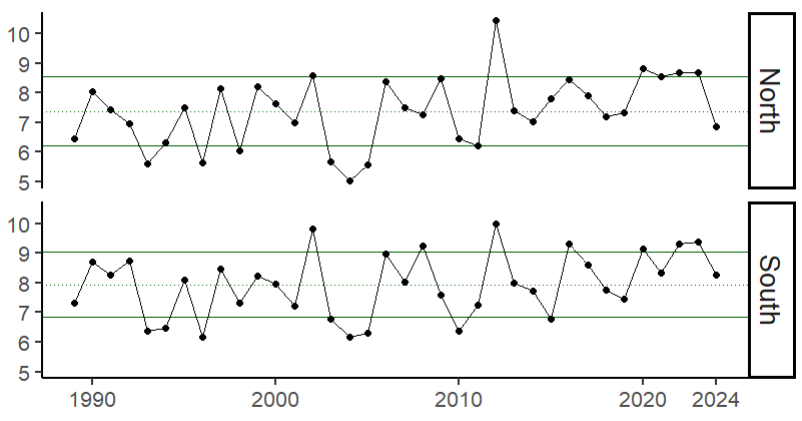
\includegraphics[width=3in, height=1.5in]{/home/atyrell/SOE_ESP_Data/bsb/docs/targets_test_files/figure-latex/unnamed-chunk-5-1.png}} & \multicolumn{1}{!{\color[HTML]{666666}\vrule width 0.75pt}>{\raggedleft}m{\dimexpr 0.75in+0\tabcolsep}!{\color[HTML]{666666}\vrule width 0.75pt}}{\textcolor[HTML]{000000}{\fontsize{10}{10}\selectfont{}}} \\

\noalign{\global\arrayrulewidth 0.75pt}\arrayrulecolor[HTML]{666666}

\hhline{|>{\arrayrulecolor[HTML]{666666}\global\arrayrulewidth=0.75pt}-|>{\arrayrulecolor[HTML]{666666}\global\arrayrulewidth=0.75pt}-|>{\arrayrulecolor[HTML]{666666}\global\arrayrulewidth=0.75pt}-|>{\arrayrulecolor[HTML]{666666}\global\arrayrulewidth=0.75pt}-|>{\arrayrulecolor[HTML]{666666}\global\arrayrulewidth=0.75pt}-}



\multicolumn{1}{!{\color[HTML]{666666}\vrule width 0.75pt}>{\cellcolor[HTML]{FFFFFF}\raggedright}m{\dimexpr 0.9in+0\tabcolsep}}{\textcolor[HTML]{000000}{\fontsize{10}{10}\selectfont{Shelf\ water\ volume\ (km3)}}} & \multicolumn{1}{!{\color[HTML]{666666}\vrule width 0.75pt}>{\cellcolor[HTML]{FFFFFF}\raggedright}m{\dimexpr 0.75in+0\tabcolsep}}{\textcolor[HTML]{000000}{\fontsize{10}{10}\selectfont{N/A\ (no\ data\ for\ 2024)}}} & \multicolumn{1}{!{\color[HTML]{666666}\vrule width 0.75pt}>{\cellcolor[HTML]{FFFFFF}\raggedright}m{\dimexpr 3in+0\tabcolsep}}{\textcolor[HTML]{000000}{\fontsize{10}{10}\selectfont{Shelf\ water\ volume\ is\ a\ proxy\ for\ suitable\ winter\ habitat;\ higher\ shelf\ water\ volume\ indicates\ less\ suitable\ habitat,\ potentially\ leading\ to\ northern\ fish\ migrating\ into\ the\ southern\ subregion.\ The\ shelf\ water\ volume\ dataset\ is\ created\ from\ in\ situ\ data,\ and\ there\ has\ been\ no\ winter\ sampling\ since\ 2021,\ highlighting\ the\ need\ for\ additional\ indicators\ to\ inform\ stock\ subunit\ mixing.}}} & \multicolumn{1}{!{\color[HTML]{666666}\vrule width 0.75pt}>{\cellcolor[HTML]{FFFFFF}\centering}m{\dimexpr 3in+0\tabcolsep}}{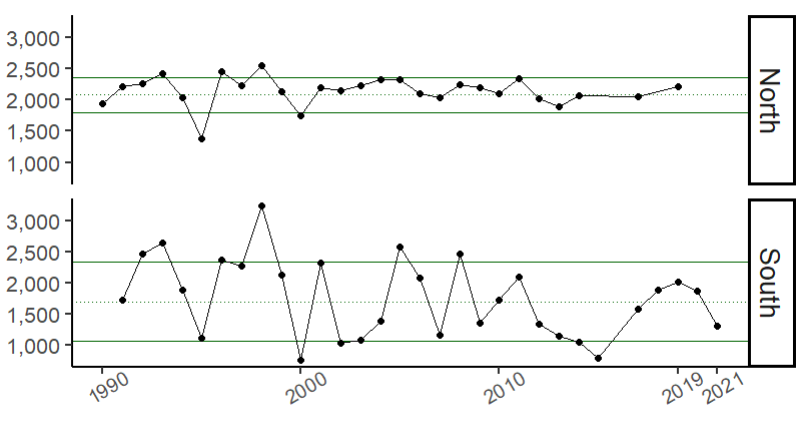
\includegraphics[width=3in, height=1.5in]{/home/atyrell/SOE_ESP_Data/bsb/docs/targets_test_files/figure-latex/unnamed-chunk-5-2.png}} & \multicolumn{1}{!{\color[HTML]{666666}\vrule width 0.75pt}>{\raggedleft}m{\dimexpr 0.75in+0\tabcolsep}!{\color[HTML]{666666}\vrule width 0.75pt}}{\textcolor[HTML]{000000}{\fontsize{10}{10}\selectfont{}}} \\

\noalign{\global\arrayrulewidth 0.75pt}\arrayrulecolor[HTML]{666666}

\hhline{|>{\arrayrulecolor[HTML]{666666}\global\arrayrulewidth=0.75pt}-|>{\arrayrulecolor[HTML]{666666}\global\arrayrulewidth=0.75pt}-|>{\arrayrulecolor[HTML]{666666}\global\arrayrulewidth=0.75pt}-|>{\arrayrulecolor[HTML]{666666}\global\arrayrulewidth=0.75pt}-|>{\arrayrulecolor[HTML]{666666}\global\arrayrulewidth=0.75pt}-}



\multicolumn{1}{!{\color[HTML]{666666}\vrule width 0.75pt}>{\cellcolor[HTML]{FFFFFF}\raggedright}m{\dimexpr 0.9in+0\tabcolsep}}{\textcolor[HTML]{000000}{\fontsize{10}{10}\selectfont{MRIP\ recreational\ trips\ (millions\ of\ annual\ trips)}}} & \multicolumn{1}{!{\color[HTML]{666666}\vrule width 0.75pt}>{\cellcolor[HTML]{FFFFFF}\raggedright}m{\dimexpr 0.75in+0\tabcolsep}}{\textcolor[HTML]{000000}{\fontsize{10}{10}\selectfont{Above\ long-term\ average}}} & \multicolumn{1}{!{\color[HTML]{666666}\vrule width 0.75pt}>{\cellcolor[HTML]{FFFFFF}\raggedright}m{\dimexpr 3in+0\tabcolsep}}{\textcolor[HTML]{000000}{\fontsize{10}{10}\selectfont{Recent\ trip\ numbers\ are\ near\ an\ all-time\ high,\ but\ have\ decreased\ from\ 2023.\ Catch\ (not\ shown)\ generally\ reflects\ trip\ patterns.\ High\ regulatory\ complexity\ is\ likely\ contributing\ to\ recreational\ fishing\ trends.}}} & \multicolumn{1}{!{\color[HTML]{666666}\vrule width 0.75pt}>{\cellcolor[HTML]{FFFFFF}\centering}m{\dimexpr 3in+0\tabcolsep}}{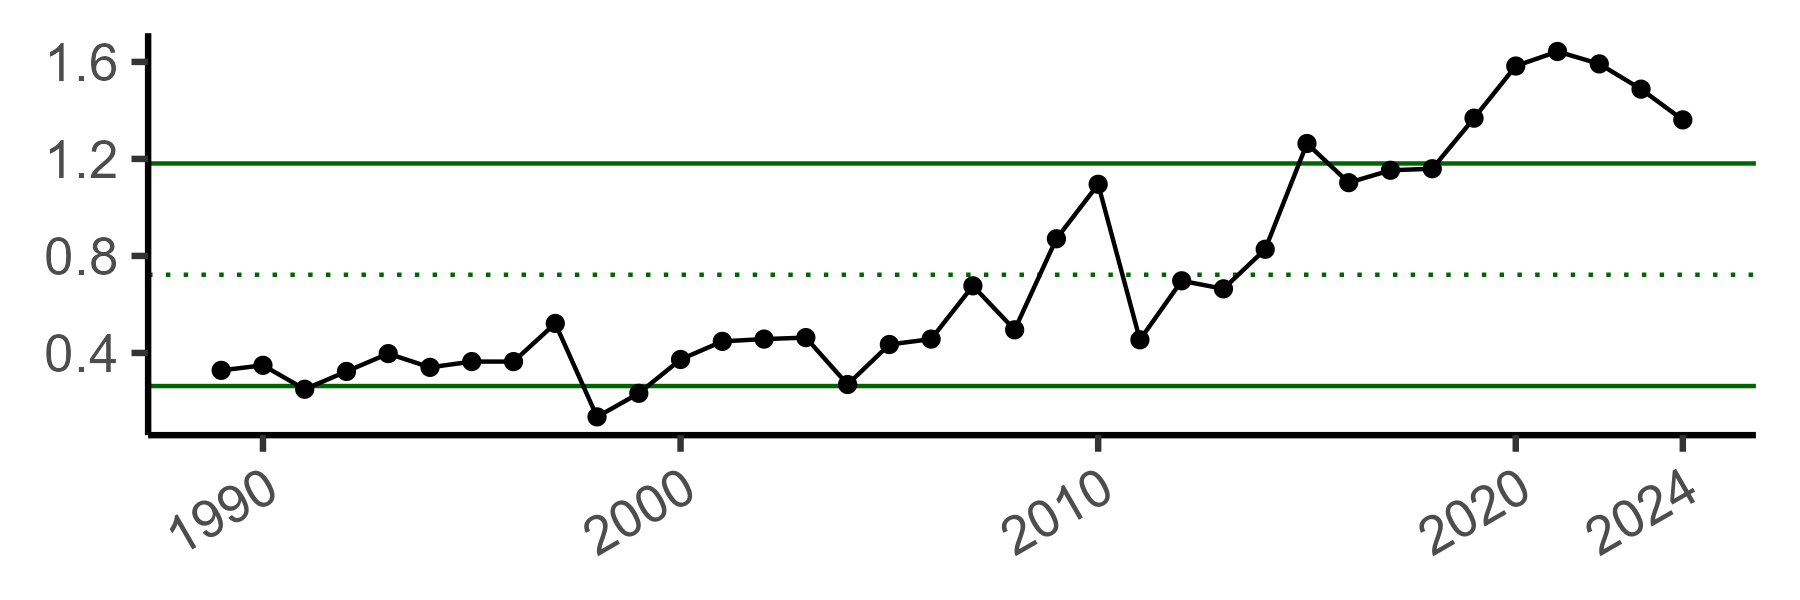
\includegraphics[width=3in, height=1in]{/home/atyrell/SOE_ESP_Data/bsb/docs/targets_test_files/figure-latex/unnamed-chunk-5-3.png}} & \multicolumn{1}{!{\color[HTML]{666666}\vrule width 0.75pt}>{\raggedleft}m{\dimexpr 0.75in+0\tabcolsep}!{\color[HTML]{666666}\vrule width 0.75pt}}{\textcolor[HTML]{000000}{\fontsize{10}{10}\selectfont{}}} \\

\noalign{\global\arrayrulewidth 0.75pt}\arrayrulecolor[HTML]{666666}

\hhline{|>{\arrayrulecolor[HTML]{666666}\global\arrayrulewidth=0.75pt}-|>{\arrayrulecolor[HTML]{666666}\global\arrayrulewidth=0.75pt}-|>{\arrayrulecolor[HTML]{666666}\global\arrayrulewidth=0.75pt}-|>{\arrayrulecolor[HTML]{666666}\global\arrayrulewidth=0.75pt}-|>{\arrayrulecolor[HTML]{666666}\global\arrayrulewidth=0.75pt}-}



\multicolumn{1}{!{\color[HTML]{666666}\vrule width 0.75pt}>{\cellcolor[HTML]{FFFFFF}\raggedright}m{\dimexpr 0.9in+0\tabcolsep}}{\textcolor[HTML]{000000}{\fontsize{10}{10}\selectfont{MRIP\ recreational\ landings\ (millions\ of\ lbs.)}}} & \multicolumn{1}{!{\color[HTML]{666666}\vrule width 0.75pt}>{\cellcolor[HTML]{FFFFFF}\raggedright}m{\dimexpr 0.75in+0\tabcolsep}}{\textcolor[HTML]{000000}{\fontsize{10}{10}\selectfont{Near\ long-term\ average}}} & \multicolumn{1}{!{\color[HTML]{666666}\vrule width 0.75pt}>{\cellcolor[HTML]{FFFFFF}\raggedright}m{\dimexpr 3in+0\tabcolsep}}{\textcolor[HTML]{000000}{\fontsize{10}{10}\selectfont{The\ recreational\ black\ sea\ bass\ fishery\ has\ a\ catch-and-release\ component,\ and\ management\ measures\ are\ being\ implemented\ to\ reduce\ recreational\ harvest.}}} & \multicolumn{1}{!{\color[HTML]{666666}\vrule width 0.75pt}>{\cellcolor[HTML]{FFFFFF}\centering}m{\dimexpr 3in+0\tabcolsep}}{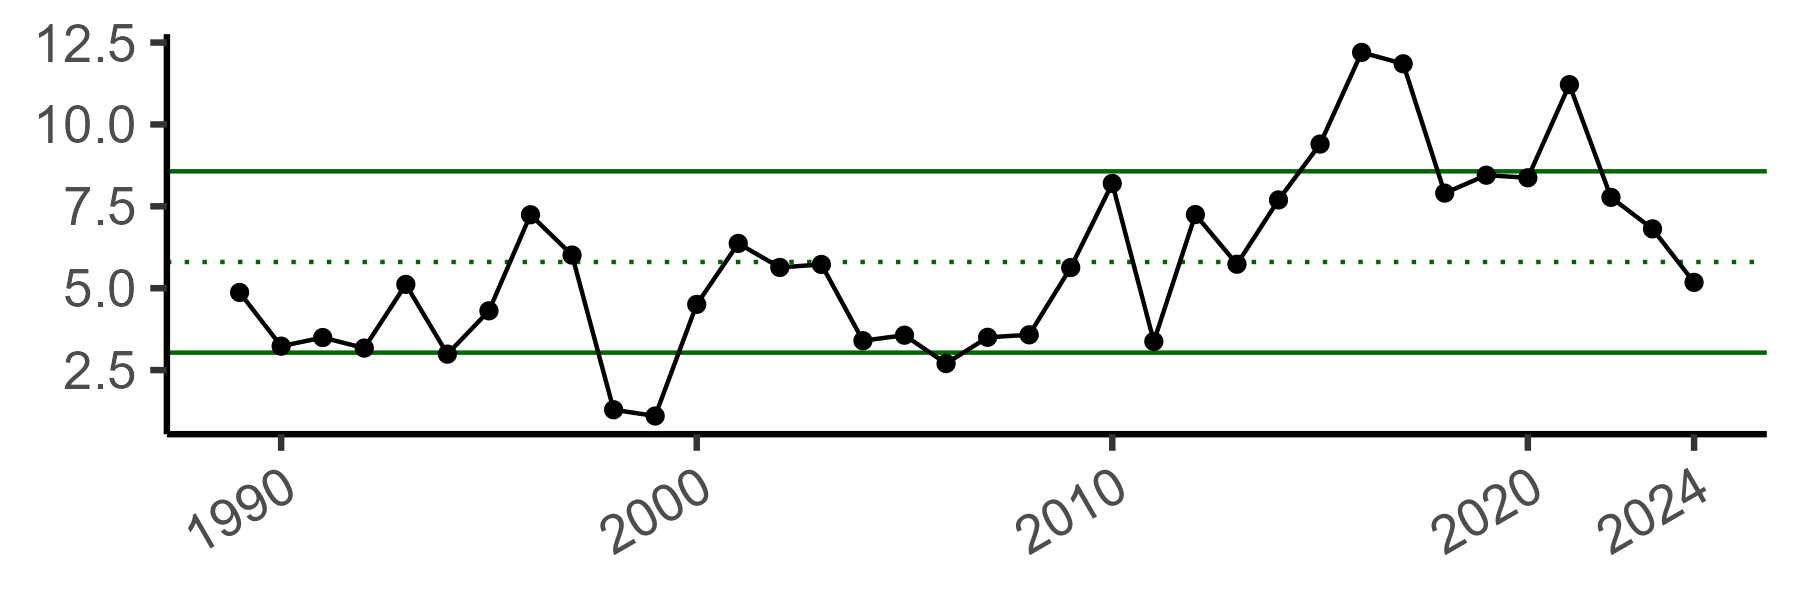
\includegraphics[width=3in, height=1in]{/home/atyrell/SOE_ESP_Data/bsb/docs/targets_test_files/figure-latex/unnamed-chunk-5-4.png}} & \multicolumn{1}{!{\color[HTML]{666666}\vrule width 0.75pt}>{\raggedleft}m{\dimexpr 0.75in+0\tabcolsep}!{\color[HTML]{666666}\vrule width 0.75pt}}{\textcolor[HTML]{000000}{\fontsize{10}{10}\selectfont{}}} \\

\noalign{\global\arrayrulewidth 0.75pt}\arrayrulecolor[HTML]{666666}

\hhline{|>{\arrayrulecolor[HTML]{666666}\global\arrayrulewidth=0.75pt}-|>{\arrayrulecolor[HTML]{666666}\global\arrayrulewidth=0.75pt}-|>{\arrayrulecolor[HTML]{666666}\global\arrayrulewidth=0.75pt}-|>{\arrayrulecolor[HTML]{666666}\global\arrayrulewidth=0.75pt}-|>{\arrayrulecolor[HTML]{666666}\global\arrayrulewidth=0.75pt}-}



\multicolumn{1}{!{\color[HTML]{666666}\vrule width 0.75pt}>{\cellcolor[HTML]{FFFFFF}\raggedright}m{\dimexpr 0.9in+0\tabcolsep}}{\textcolor[HTML]{000000}{\fontsize{10}{10}\selectfont{Commercial\ revenue\ per\ vessel\ (2024\ USD)}}} & \multicolumn{1}{!{\color[HTML]{666666}\vrule width 0.75pt}>{\cellcolor[HTML]{FFFFFF}\raggedright}m{\dimexpr 0.75in+0\tabcolsep}}{\textcolor[HTML]{000000}{\fontsize{10}{10}\selectfont{Above\ long-term\ average}}} & \multicolumn{1}{!{\color[HTML]{666666}\vrule width 0.75pt}>{\cellcolor[HTML]{FFFFFF}\raggedright}m{\dimexpr 3in+0\tabcolsep}}{\textcolor[HTML]{000000}{\fontsize{10}{10}\selectfont{Commercial\ revenue\ per\ vessel\ follows\ an\ overall\ increasing\ trend\ most\ likely\ driven\ by\ the\ continued\ decline\ of\ active\ vessels\ and\ an\ overall\ increase\ in\ total\ commercial\ landed\ pounds\ over\ the\ past\ decade.\  }}} & \multicolumn{1}{!{\color[HTML]{666666}\vrule width 0.75pt}>{\cellcolor[HTML]{FFFFFF}\centering}m{\dimexpr 3in+0\tabcolsep}}{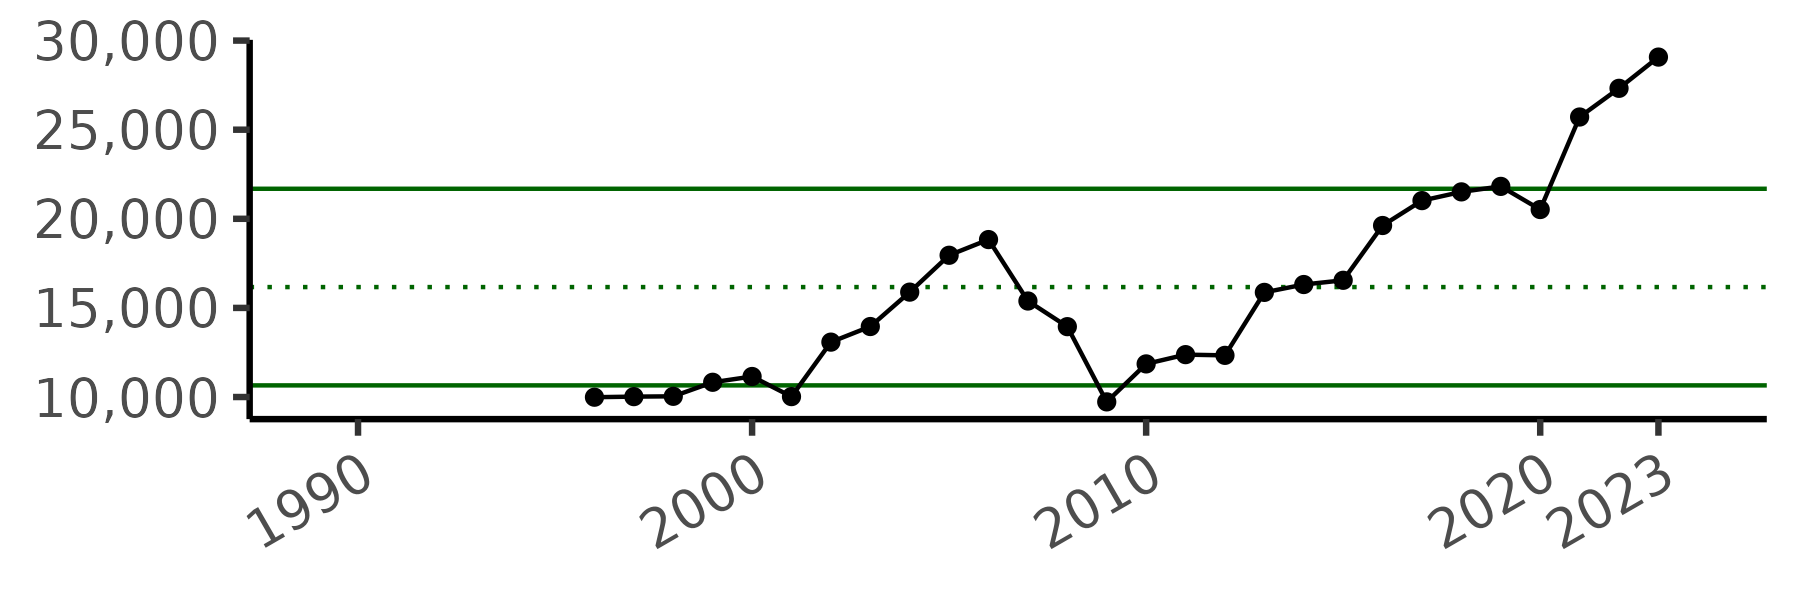
\includegraphics[width=3in, height=1in]{/home/atyrell/SOE_ESP_Data/bsb/docs/targets_test_files/figure-latex/unnamed-chunk-5-5.png}} & \multicolumn{1}{!{\color[HTML]{666666}\vrule width 0.75pt}>{\raggedleft}m{\dimexpr 0.75in+0\tabcolsep}!{\color[HTML]{666666}\vrule width 0.75pt}}{\textcolor[HTML]{000000}{\fontsize{10}{10}\selectfont{}}} \\

\noalign{\global\arrayrulewidth 0.75pt}\arrayrulecolor[HTML]{666666}

\hhline{|>{\arrayrulecolor[HTML]{666666}\global\arrayrulewidth=0.75pt}-|>{\arrayrulecolor[HTML]{666666}\global\arrayrulewidth=0.75pt}-|>{\arrayrulecolor[HTML]{666666}\global\arrayrulewidth=0.75pt}-|>{\arrayrulecolor[HTML]{666666}\global\arrayrulewidth=0.75pt}-|>{\arrayrulecolor[HTML]{666666}\global\arrayrulewidth=0.75pt}-}



\multicolumn{1}{!{\color[HTML]{666666}\vrule width 0.75pt}>{\cellcolor[HTML]{FFFFFF}\raggedright}m{\dimexpr 0.9in+0\tabcolsep}}{\textcolor[HTML]{000000}{\fontsize{10}{10}\selectfont{Number\ of\ commercial\ vessels\ (\#)}}} & \multicolumn{1}{!{\color[HTML]{666666}\vrule width 0.75pt}>{\cellcolor[HTML]{FFFFFF}\raggedright}m{\dimexpr 0.75in+0\tabcolsep}}{\textcolor[HTML]{000000}{\fontsize{10}{10}\selectfont{Below\ long-term\ average}}} & \multicolumn{1}{!{\color[HTML]{666666}\vrule width 0.75pt}>{\cellcolor[HTML]{FFFFFF}\raggedright}m{\dimexpr 3in+0\tabcolsep}}{\textcolor[HTML]{000000}{\fontsize{10}{10}\selectfont{The\ number\ of\ active\ vessels\ has\ been\ decreasing\ since\ 2017,\ which\ could\ impact\ revenue\ distributions\ and\ fleet\ composition. }}} & \multicolumn{1}{!{\color[HTML]{666666}\vrule width 0.75pt}>{\cellcolor[HTML]{FFFFFF}\centering}m{\dimexpr 3in+0\tabcolsep}}{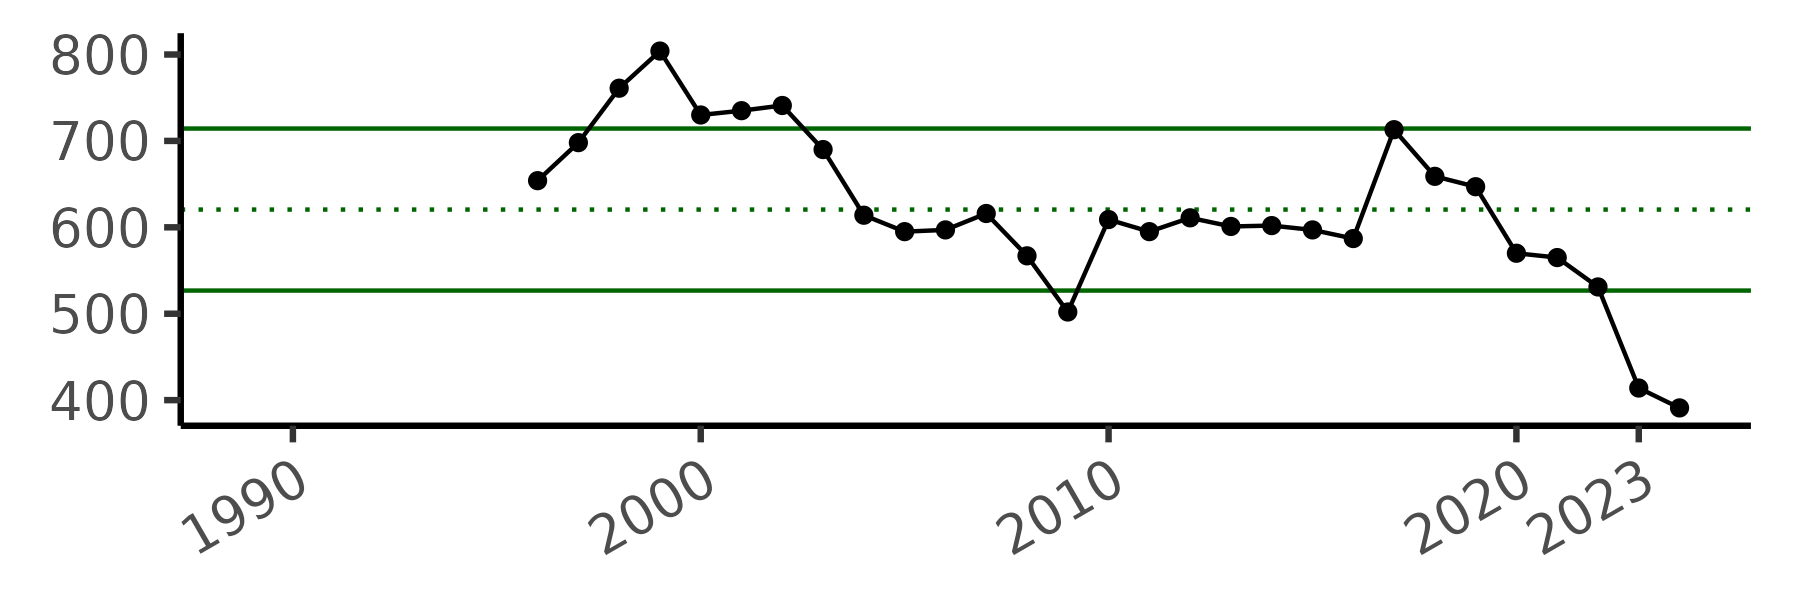
\includegraphics[width=3in, height=1in]{/home/atyrell/SOE_ESP_Data/bsb/docs/targets_test_files/figure-latex/unnamed-chunk-5-6.png}} & \multicolumn{1}{!{\color[HTML]{666666}\vrule width 0.75pt}>{\raggedleft}m{\dimexpr 0.75in+0\tabcolsep}!{\color[HTML]{666666}\vrule width 0.75pt}}{\textcolor[HTML]{000000}{\fontsize{10}{10}\selectfont{}}} \\

\noalign{\global\arrayrulewidth 0.75pt}\arrayrulecolor[HTML]{666666}

\hhline{|>{\arrayrulecolor[HTML]{666666}\global\arrayrulewidth=0.75pt}-|>{\arrayrulecolor[HTML]{666666}\global\arrayrulewidth=0.75pt}-|>{\arrayrulecolor[HTML]{666666}\global\arrayrulewidth=0.75pt}-|>{\arrayrulecolor[HTML]{666666}\global\arrayrulewidth=0.75pt}-|>{\arrayrulecolor[HTML]{666666}\global\arrayrulewidth=0.75pt}-}



\end{longtable}



\arrayrulecolor[HTML]{000000}

\global\setlength{\arrayrulewidth}{\Oldarrayrulewidth}

\global\setlength{\tabcolsep}{\Oldtabcolsep}

\renewcommand*{\arraystretch}{1}

\centering

Please contact \url{nefsc.esp.leads@noaa.gov} with any questions or
comments.

\vspace{0.5cm}
\raggedright

Commercial data were derived from the commercial dealer database hosted
at the Greater Atlantic Regional Office. All dollar values have been
adjusted to 2024 real dollars using the
\href{https://fred.stlouisfed.org/series/GDPDEF}{Gross Domestic Implicit
Price Deflator}.

\end{document}
